\documentclass{beamer}

\mode<presentation> {

%\usetheme{default}
%\usetheme{AnnArbor}
%\usetheme{Antibes}
%\usetheme{Bergen}
%\usetheme{Berkeley}
%\usetheme{Berlin}
%\usetheme{Boadilla}
%\usetheme{CambridgeUS}
%\usetheme{Copenhagen}
%\usetheme{Darmstadt}
% \usetheme{Dresden}
%\usetheme{Frankfurt}
\usetheme{Goettingen}
%\usetheme{Hannover}
%\usetheme{Ilmenau}
%\usetheme{JuanLesPins}
%\usetheme{Luebeck}
% \usetheme{Madrid}
%\usetheme{Malmoe}
%\usetheme{Marburg}
%\usetheme{Montpellier}
%\usetheme{PaloAlto}
%\usetheme{Pittsburgh}
%\usetheme{Rochester}
%\usetheme{Singapore}
%\usetheme{Szeged}
%\usetheme{Warsaw}


%\usecolortheme{albatross}
%\usecolortheme{beaver}
%\usecolortheme{beetle}
%\usecolortheme{crane}
%\usecolortheme{dolphin}
%\usecolortheme{dove}
%\usecolortheme{fly}
%\usecolortheme{lily}
%\usecolortheme{orchid}
%\usecolortheme{rose}
%\usecolortheme{seagull}
%\usecolortheme{seahorse}
%\usecolortheme{whale}
%\usecolortheme{wolverine}

%\setbeamertemplate{footline} % To remove the footer line in all slides uncomment this line
%\setbeamertemplate{footline}[page number] % To replace the footer line in all slides with a simple slide count uncomment this line

%\setbeamertemplate{navigation symbols}{} % To remove the navigation symbols from the bottom of all slides uncomment this line
}

\usepackage{graphicx} % Allows including images
\usepackage{booktabs} % Allows the use of \toprule, \midrule and \bottomrule in tables
\usepackage{amsfonts}
\usepackage{mathrsfs, bbold}
\usepackage{amsmath,amssymb,graphicx}
\usepackage{mathtools} % gather
\usepackage[export]{adjustbox} % right-aligned graphics

% tikz?
\usepackage{tikz}
\usetikzlibrary{arrows, shapes}


\usepackage[style=authortitle,backend=bibtex]{biblatex}
%\usepackage[backend=biber,style=numeric-comp,sorting=none]{biblatex}
\addbibresource{references.bib}

%----------------------------------------------------------------------------------------
%	TITLE PAGE
%----------------------------------------------------------------------------------------

\title["10"]{10: Introduction to Bayesian Computation}

\author{Taylor} 
\institute[UVA] 
{
University of Virginia \\
\medskip
\textit{} 
}
\date{} 
    
\begin{document}
%----------------------------------------------------------------------------------------

\begin{frame}
\titlepage 
\end{frame}

%----------------------------------------------------------------------------------------


\begin{frame}
\tableofcontents
\end{frame}

%----------------------------------------------------------------------------------------
\section{Introduction}

\begin{frame}
\frametitle{Introduction}

This chapter gives an overview for how to approximate intractable quantities such as posterior expectations and predictions. 

\end{frame}

%----------------------------------------------------------------------------------------
\begin{frame}
\frametitle{Definitions}

{\bf Numerical integration} methods approximate integrals. 
\newline

These methods can be loosely categorized as either {\bf stochastic} or {\bf deterministic} (e.g. quadrature methods).


\end{frame}


%----------------------------------------------------------------------------------------
\begin{frame}
\frametitle{Deterministic Methods}

{\bf Deterministic methods} don't draw samples, and instead approximate the integral by summing up approximate volumes:
\[
E[h(\theta) \mid y] = \int h(\theta) p(\theta \mid y) \text{d}\theta \approx \frac{1}{S} \sum_{s=1}^S w_s h(\theta^s)p(\theta^s \mid y)
\]

\end{frame}
%----------------------------------------------------------------------------------------
\begin{frame}[fragile]
\frametitle{Approximating the posterior on a grid}

We used this method earlier for the rat tumor example!
\newline

Given that we can evaluate the unnormalized target $p(\theta, y) = p(y \mid \theta)p(\theta)$, we choose a nonrandom grid of points (think \verb|seq|) $\theta_1, \ldots, \theta_S$, and then we approximate the the continuous posterior with a discrete random variable with pmf equal to
\[
\tilde{p}(\theta_j \mid y) = \frac{p(y \mid \theta_j)p(\theta_j)}{\sum_{s=1}^S p(y \mid \theta_s)p(\theta_s) }
\]
for any $\theta_j \in \{\theta_1, \ldots, \theta_S\}$. Then
\newline

$$
E[h(\theta) \mid y] \approx \sum_{j=1}^S h(\theta_j)\tilde{p}(\theta_j \mid y) .
$$

\end{frame}
%----------------------------------------------------------------------------------------
\begin{frame}
\frametitle{Stochastic Methods}

{\bf Stochastic methods} involve sample averages of simulated draws from some distribution. There are {\bf many} ways to do this, but here are a couple examples that we've seen:
\[
E[h(\theta) \mid y] = \int h(\theta) p(\theta \mid y) \text{d}\theta \approx \frac{1}{S} \sum_{s=1}^S h(\theta^s)
\]
with $\theta^s \sim p(\theta \mid y)$, or
\[
E[h(\tilde{y}) \mid y] = \int h(\tilde{y}) p(\tilde{y} \mid y) \text{d} \tilde{y} \approx \frac{1}{S} \sum_{s=1}^S h(\tilde{y}^s)
\]
with $\tilde{y} \sim p(\tilde{y} \mid y)$

\end{frame}

%----------------------------------------------------------------------------------------
\begin{frame}
\frametitle{Stochastic Methods}

Drawing $\tilde{y}$ samples can be done in a two-stage way:
\begin{enumerate}
\item draw $\theta^s \sim p(\theta \mid y)$
\item draw $\tilde{y}^s \sim p(\tilde{y} \mid \theta^s)$
\end{enumerate}
\pause

If you can derive $E\left( h(\tilde{y}) \mid \theta \right)$, you should probably use a Rao-Blackwellized procedure:
\[
E[h(\tilde{y}) \mid y] = E[E\left( h(\tilde{y}) \mid \theta \right) \mid y] \approx \frac{1}{S} \sum_{s=1}^S E\left( h(\tilde{y}) \mid \theta^s \right)
\]
with $\theta^s \sim p(\theta \mid y)$


\end{frame}


%----------------------------------------------------------------------------------------
\begin{frame}[fragile]
\frametitle{The general setup}

From now on we will write the posterior in terms of an unnormalized density $q(\theta \mid y)$. In other words:
\[
p(\theta \mid y) = \frac{q(\theta \mid y)}{ \int q(\theta \mid y) \text{d}\theta}
\]

Most (maybe all) of the sampling techniques will assume that we can't evaluate $p(\theta \mid y)$, but that we can evaluate $q(\theta \mid y)$

\end{frame}


%----------------------------------------------------------------------------------------
\section{Accept-Reject Sampling}

\begin{frame}[fragile]
\frametitle{Rejection Sampling aka Accept-Reject sampling}

Setup
\begin{enumerate}
\item $p(\theta \mid y)$ the target, posterior
\item $q(\theta \mid y) = p(y \mid \theta) p(\theta)$ the unnormalized target
\item $g(\theta)$ the ``instrumental" or ``proposal" distribution
\item need $q(\theta \mid y) / g(\theta) \le M$ uniformly
\item need $g \gg q$ i.e. the proposal ``dominates" your target (won't divide by $0$)
\end{enumerate}
We are free to choose our own $g(\theta)$. For the time being, we assume that $\int g(\theta) \text{d}\theta = 1$.

\end{frame}
%----------------------------------------------------------------------------------------
\begin{frame}[fragile]
\frametitle{Rejection Sampling aka Accept-Reject sampling}


To (potentially) produce one draw:
\begin{enumerate}
\item propose the draw $\theta^s \sim g(\theta)$
\item accept $\theta^s$ with probability $\frac{q(\theta^s \mid y) }{ g(\theta^s)  M }$
\end{enumerate}
\pause

Note this is the same as
\begin{enumerate}
\item propose the draw $\theta^s \sim g(\theta)$
\item draw $U \sim \text{Uniform}(0,1]$
\item accept $\theta^s$ if $U < q(\theta^s \mid y) / \{ g(\theta^s)  M\}$
\end{enumerate}


\end{frame}
%----------------------------------------------------------------------------------------
\begin{frame}[fragile]
\frametitle{Proof }

\begin{align*}
P\left( \theta \le t \bigg\rvert U \le \frac{q(\theta \mid y)}{M g(\theta) } \right) 
&= \frac{P\left( \theta \le t , U \le \frac{q(\theta \mid y)}{M g(\theta) } \right)}{P\left(U \le \frac{q(\theta \mid y)}{M g(\theta) } \right)} \\
&= \frac{\int_{-\infty}^t \int_0^{ \frac{q(\theta \mid y)}{M g(\theta) } }g(\theta)1 \text{d}u \text{d}\theta }{ \int_{-\infty}^{\infty} \int_0^{ \frac{q(\theta \mid y)}{M g(\theta) } }g(\theta)1 \text{d}u \text{d}\theta } \\
&= \frac{\int_{-\infty}^t g(\theta)\frac{q(\theta \mid y)}{M g(\theta) }  \text{d}\theta }{ \int_{-\infty}^{\infty} g(\theta)  \frac{q(\theta \mid y)}{M g(\theta) } \text{d}\theta } \\
&= \frac{\int_{-\infty}^t q(\theta \mid y)  \text{d}\theta }{ \int_{-\infty}^{\infty}  q(\theta \mid y)\text{d}\theta } \\
&= P(\theta \le t \mid y).
\end{align*}
\end{frame}


%----------------------------------------------------------------------------------------
\begin{frame}[fragile]
\frametitle{Example 1}

Assume $y \sim \text{Normal}(\theta,1)$, and $p(\theta) = \frac{1}{\pi(1+\theta^2)}$. 
Our goal is to draw from
\begin{align*}
p(\theta \mid y) &\propto q(\theta\mid y) \\
&= p(y \mid \theta) p(\theta) \\
&= \frac{1}{\sqrt{2\pi}} \exp\left[-\frac{1}{2} (y-\theta)^2 \right] \frac{1}{\pi(1+\theta^2)} \\
&\propto \exp\left[-\frac{(\theta - y)^2}{2} - \log(1 + \theta^2) \right],
\end{align*}


\end{frame}

%----------------------------------------------------------------------------------------
\begin{frame}[fragile]
\frametitle{Example 1}

Let's assume that we want to use our prior distribution as a proposal: $g(\theta) = p(\theta)$. Then we have to find $M$:
\begin{align*}
\frac{q(\theta\mid y)}{g(\theta)} &= \frac{p(y \mid \theta) p(\theta)}{p(\theta)} \\
&= p(y \mid \theta) \\
&= \frac{1}{\sqrt{2\pi}} \exp\left[-\frac{1}{2} (y-\theta)^2 \right] \\
&\le \frac{1}{\sqrt{2\pi}} \overset{\text{def}}{=} M
\end{align*}

Our acceptance probability for draw $\theta^s$ is then
\[
q(\theta^s \mid y) / \{ g(\theta^s)  M\} = p(y \mid \theta^s) / M = \exp\left[-\frac{1}{2} (y-\theta^s)^2 \right]
\]


\end{frame}
%----------------------------------------------------------------------------------------
\begin{frame}[fragile]
\frametitle{Rejection Sampling aka Accept-Reject sampling}

Generally a good strategy is work with logarithms, and then exponentiate as late as possible.
\begin{verbatim}
y <- 2 # fake data
num_trials <- 1000
theta_proposals <- rt(num_trials, 1)
us <- runif(num_trials, min = 0, max = 1)
log_accept_prob <- function(theta){
  -.5*(y - theta)^2
}
probs <- exp(log_accept_prob(theta_proposals))
accepts <- ifelse(us < probs, TRUE, FALSE)
hist(theta_proposals[accepts]) # only the accepted draws
#hist(theta_proposals) # all draws!
\end{verbatim}

\end{frame}

%----------------------------------------------------------------------------------------
\section{Importance Sampling}
\begin{frame}[fragile]
\frametitle{Importance Sampling}

{\bf importance sampling} also involves ratios like the previous algorithm. However, instead of using those ratios to either accept or discard samples, it uses the ratios to weight samples. 
\newline


\end{frame}

%----------------------------------------------------------------------------------------
\begin{frame}[fragile]
\frametitle{Importance Sampling}

\begin{center}
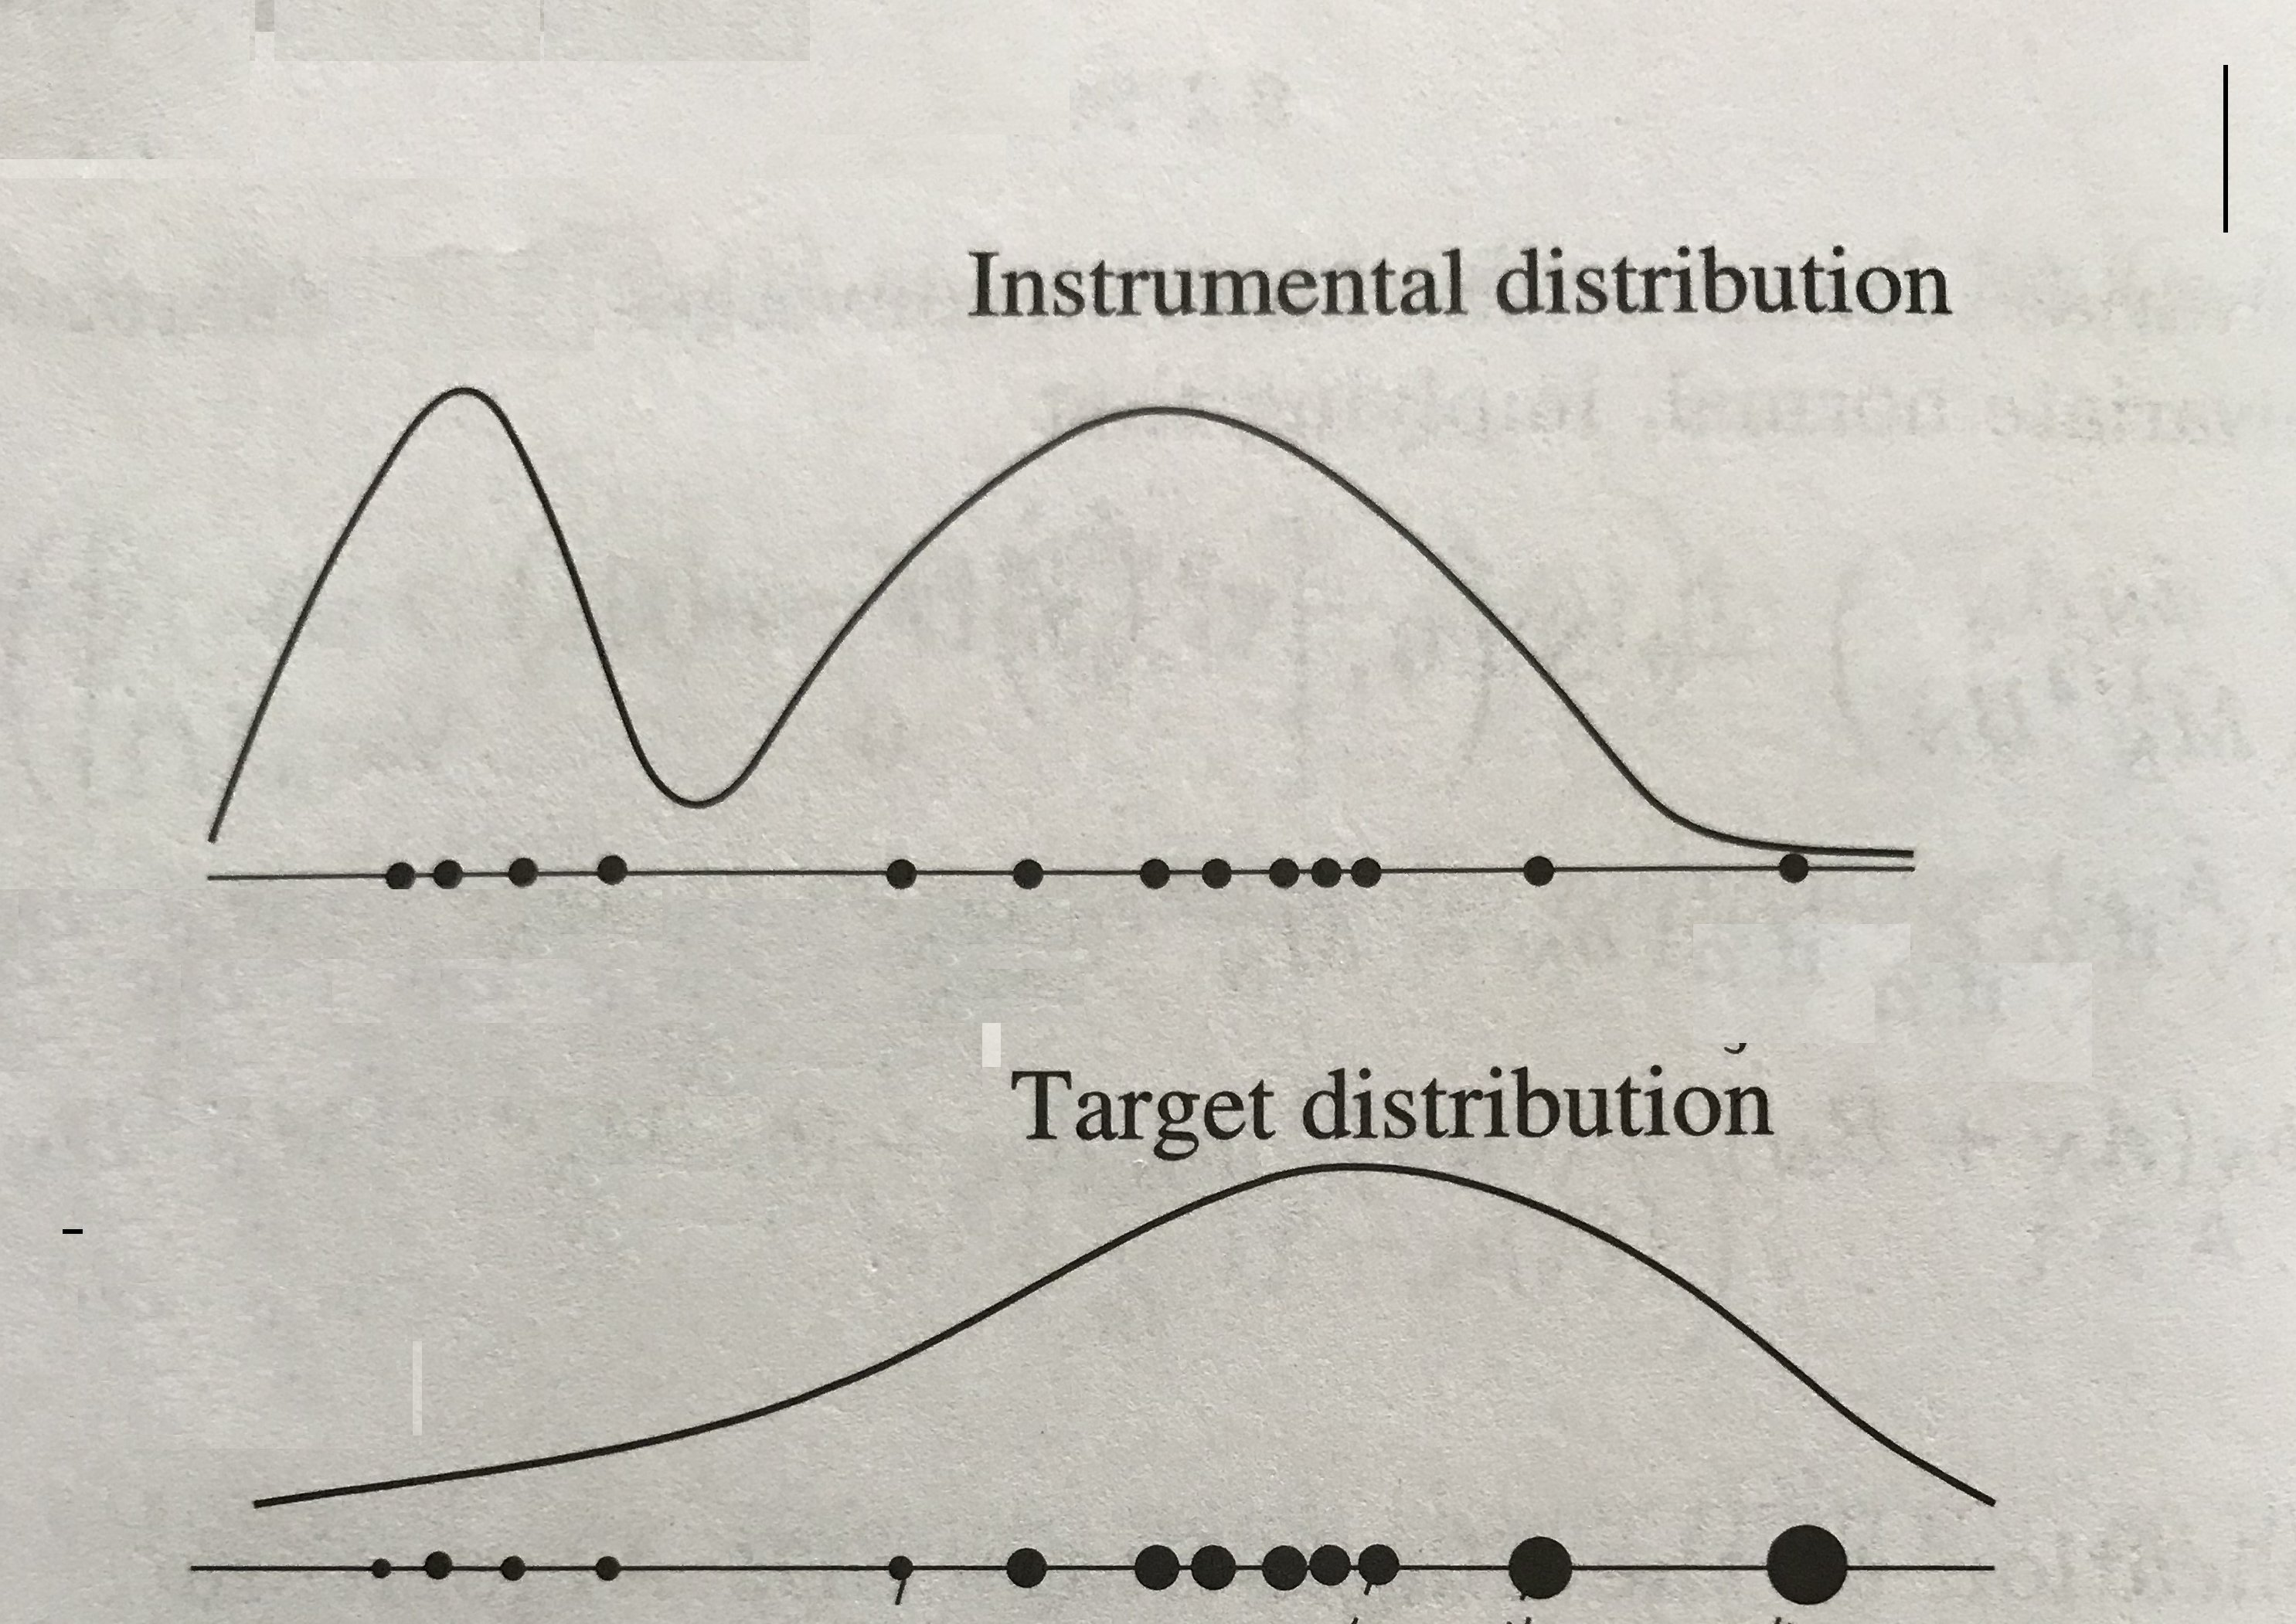
\includegraphics[width=90mm]{is.jpg}
\end{center}
Original, unedited image is from \url{https://www.springer.com/us/book/9780387402642}

\end{frame}
%----------------------------------------------------------------------------------------
\begin{frame}[fragile]
\frametitle{Importance Sampling}

Setup
\begin{enumerate}
\item $p(\theta \mid y)$ the target, posterior
\item $q(\theta \mid y) = p(y \mid \theta) p(\theta)$ the unnormalized target
\item $g(\theta)$ the ``instrumental" or ``proposal" distribution
\item $g \gg q$ i.e. the proposal dominates your target 
\end{enumerate}
We are free to choose our own $g(\theta)$. For the time being, we assume that $\int g(\theta) \text{d}\theta = 1$.


\end{frame}


%----------------------------------------------------------------------------------------
\begin{frame}[fragile]
\frametitle{Importance Sampling}

Algorithm: for each iteration $s$
\begin{enumerate}
\item draw $\theta^s \sim g(\theta)$
\item calculate unnormalized weight $\tilde{w}(\theta^s) = \frac{q(\theta^s \mid y)}{g(\theta^s)}$
\item calculate normalized weights $w(\theta^s) = \tilde{w}(\theta^s)/\sum_r \tilde{w}(\theta^r)$
\end{enumerate}
Final calculation: 
$$
E_q[h(\theta) \mid y] \approx \sum_s w(\theta^s) h(\theta^s)
$$
\end{frame}

%----------------------------------------------------------------------------------------
\begin{frame}[fragile]
\frametitle{Importance Sampling}

Motivation:
\begin{align*}
E_q[h(\theta) \mid y] &= \int h(\theta) p(\theta \mid y) \text{d}\theta \\
&= \frac{\int h(\theta) q(\theta \mid y) \text{d}\theta }{\int q(\theta \mid y) \text{d}\theta } \\
&= \frac{\int h(\theta) \frac{q(\theta \mid y)}{g(\theta)}g(\theta) \text{d}\theta }{\int \frac{q(\theta \mid y)}{g(\theta)}g(\theta) \text{d}\theta } 
\end{align*}
\newline
\pause

So first:
\[
\frac{1}{S}\sum_{s=1}^S \frac{q(\theta^s \mid y)}{g(\theta^s)} \to E_g\left[\frac{q(\theta \mid y)}{g(\theta)} \right] = \int \frac{q(\theta \mid y)}{g(\theta)} g(\theta) \text{d}\theta = \int q(\theta \mid y) \text{d}\theta
\]

\end{frame}

%----------------------------------------------------------------------------------------
\begin{frame}[fragile]
\frametitle{Importance Sampling}

\begin{enumerate}
\item $E_q[h(\theta) \mid y] = \frac{\int h(\theta) q(\theta \mid y) \text{d}\theta }{\int q(\theta \mid y) \text{d}\theta } $
\item $\frac{1}{S}\sum_{s=1}^S \frac{q(\theta^s \mid y)}{g(\theta^s)} \to \int q(\theta \mid y) \text{d}\theta$ ( for the denominator)
\end{enumerate}
And second:
\[
\frac{1}{S}\sum_{s=1}^S h(\theta^s) \frac{q(\theta^s \mid y)}{g(\theta^s)} \to E_g\left[h(\theta)\frac{q(\theta \mid y)}{g(\theta)} \right] = \int h(\theta)q(\theta \mid y) \text{d}\theta
\]
which converges to the numerator

\end{frame}

%----------------------------------------------------------------------------------------
\begin{frame}[fragile]
\frametitle{Importance Sampling}

\begin{enumerate}
\item $E_q[h(\theta) \mid y] = \frac{\int h(\theta) q(\theta \mid y) \text{d}\theta }{\int q(\theta \mid y) \text{d}\theta } $
\item $\frac{1}{S}\sum_{s=1}^S \frac{q(\theta^s \mid y)}{g(\theta^s)} \to \int q(\theta \mid y) \text{d}\theta$ 
\item $\frac{1}{S}\sum_{s=1}^S h(\theta^s) \frac{q(\theta^s \mid y)}{g(\theta^s)} \to \int h(\theta)q(\theta \mid y) \text{d}\theta$
\end{enumerate}

So finally
\[
\sum_{i=1}^S w(\theta^s) h(\theta^s)
=
\frac{
\sum_{s=1}^S h(\theta^s) \frac{q(\theta^s \mid y)}{g(\theta^s)}}{
\sum_{r=1}^S \frac{q(\theta^{r} \mid y)}{g(\theta^{r})}  
}
=
\frac{
\frac{1}{S}\sum_{s=1}^S h(\theta^s) \frac{q(\theta^s \mid y)}{g(\theta^s)}}{
\frac{1}{S}\sum_{r=1}^S \frac{q(\theta^{r} \mid y)}{g(\theta^{r})}  
}
\to E[h(\theta) \mid y]
\]
where $w(\theta^s) = \frac{q(\theta^s \mid y)}{g(\theta^s)} \bigg/ \sum_{r=1}^S \frac{q(\theta^{r} \mid y)}{g(\theta^{r})}  $ are the self-normalized weights

\end{frame}


%----------------------------------------------------------------------------------------
\begin{frame}[fragile]
\frametitle{Example 2}

Assume $y \sim \text{Normal}(\theta,1)$, and $p(\theta) = \frac{1}{\pi(1+\theta^2)}$. Approximate $E_q[\theta \mid y]$ using proposal $g(\theta) = p(\theta)$.
\newline
\pause

If we sample from $g(\theta) = p(\theta) = \frac{1}{\pi(1+\theta^2)}$ then the unnormalized weights are
\begin{align*}
\tilde{w}(\theta^s) &= \frac{ q(\theta^s \mid y)}{g(\theta^s)}  \\
&= p(y \mid \theta^s )  \\
&= \frac{1}{\sqrt{2\pi}} \exp\left[-\frac{1}{2} (y-\theta^s)^2 \right] 
\end{align*}
\pause

then normalize these...

\end{frame}

%----------------------------------------------------------------------------------------
\begin{frame}[fragile]
\frametitle{Example 2}


\begin{verbatim}
y <- 2 # fake data
num_samples <- 1000000
theta_draws <- rt(num_samples , 1)
log_unnorm_weight <- function(theta){ 
  # sqrt(2pi) because it will cancel out 
  -.5*(y - theta)^2
}
lunws <- log_unnorm_weight(theta_draws)
norm_weights <- exp(lunws)/sum(exp(lunws))
sum(norm_weights * theta_draws)
hist(norm_weights)
\end{verbatim}


\end{frame}



% %----------------------------------------------------------------------------------------
% \begin{frame}[fragile]
% \frametitle{Example 2}
% 
% Before I show you some sample code: using the {\bf log-sum-exp} trick becomes necessary when you have a lot of samples.
% \newline
% 
% Assume $l_1, l_2, \ldots, l_S$ are your unnormalized log weights, the bad way to calculate each log-normalized-weight is 
% \[
% \log w_s = \log \tilde{w}_s - \log \sum \tilde{w}_s = \log\left[\exp(l_s)\right] - \log \left[ \sum_{r} \exp(l_r) \right]
% \]
% because many $l_r$ will be so close to $-\infty$ that exponentiating them will round them down to $0$. 
% 
% 
% \end{frame}
% 
% %----------------------------------------------------------------------------------------
% \begin{frame}[fragile]
% \frametitle{Example 2}
% 
% Instead:
% 
% 
% \begin{align*}
% &\log\left[\exp(l_s)\right] - \log \left[ \sum_{r} \exp(l_r) \right] \\
% &= \log\left[\exp(l_s-m)e^m\right] - \log \left[ \sum_{r} \exp(l_r-m)e^m \right] \\
% &= \log\left[\exp(l_s - m)\right]  - \log \left[ \sum_{r} \exp(l_r - m) \right]
% \end{align*}
% subtracting a negative $m$ will move many log weights closer to $0$ and save a lot of them from being exponentiated to $0$!
% 
% 
% \end{frame}

%----------------------------------------------------------------------------------------
\begin{frame}[fragile]
\frametitle{Example 2}

The choice of proposal is very important. In a HW problem, you will derive the following using the delta method:
\newline

\begin{align*}
\operatorname{Var}_g \left( \sum_{s=1}^S w(\theta^s) h(\theta^s) \right) &\approx \frac{1}{S} E_g\left[  \underbrace{ \left(\frac{\tilde{w}(\theta)}{ E_g[\tilde{w}(\theta)] }\right)^2 }_{\text{!} } (h(\theta) - E_q[h(\theta) ] )^2 \right]    \\
\end{align*}

Beware of proposals that have tails that are thin relative to the target!

\end{frame}

%----------------------------------------------------------------------------------------
\begin{frame}[fragile]
\frametitle{Example 2}

\begin{center}
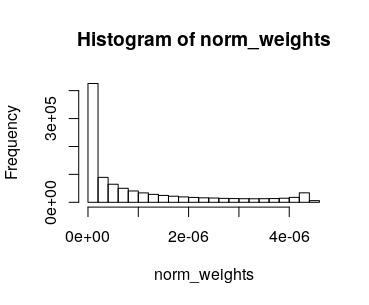
\includegraphics[width=100mm]{is_weights.png}
\end{center}

\end{frame}


%----------------------------------------------------------------------------------------
\begin{frame}[fragile]
\frametitle{Example 2}

Beware of bad proposal distributions!
\newline

A sample estimator of this approximate variance is
\[
\sum_{s=1}^S w(\theta^s) \left( h(\theta^s) - \hat{E}[h(\theta)]  \right)^2
\]
where $\hat{E}[h(\theta)] = \sum_s w(\theta^s)h(\theta^s)$. 
\newline

Note the weights aren't the same for each sample, like a ``standard" estimation of the sample variance.

\end{frame}

%----------------------------------------------------------------------------------------
\begin{frame}[fragile]
\frametitle{Example 2}

\begin{verbatim}
y <- 2 # fake data
log_unnorm_weight <- function(theta){ 
  # sqrt(2pi) because it will cancel out 
  -.5*(y - theta)^2 }
getISEstimator <- function(num_samples){
  theta_draws <- rt(num_samples , 1)
  lunws <- log_unnorm_weight(theta_draws)
  norm_weights <- exp(lunws)/sum(exp(lunws))
  estimator <- sum(norm_weights * theta_draws)
  list("estimate" = estimator, 
       "approx_var" = 
       sum( norm_weights*(theta_draws - estimator)^2) ) }
# two ways to calculate standard errors
num_samps_per_estimate <- 10
sqrt(getISEstimator(num_samps_per_estimate)$approx_var)  
sd(replicate(1000, 
    getISEstimator(num_samps_per_estimate)$estimate)) 
\end{verbatim}


\end{frame}

% %----------------------------------------------------------------------------------------
% \begin{frame}[fragile]
% \frametitle{Example 2}
% 
% \begin{verbatim}
% hist(
%   replicate(1000, 
%             getISEstimator(num_samps_per_estimate)$estimate),
%   xlab = "IS estimate",
%   main = "distribution of IS estimate") 
% \end{verbatim}
% 
% 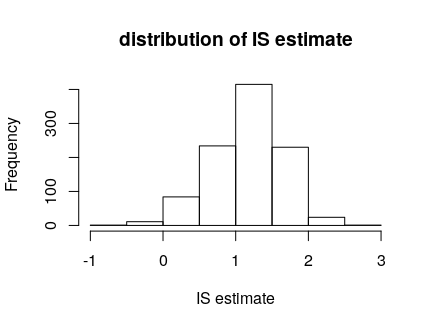
\includegraphics[width=70mm]{is1_hist.png}
% 
% 
% \end{frame}


%----------------------------------------------------------------------------------------
\begin{frame}[fragile]
\frametitle{Effective Sample Size}

Effective sample size calculations use a second order delta method. 
\newline

One form is 
$$
\textrm{ESS} = \frac{S}{1 + \textrm{Var}_g(W)}.
$$
and the other form is 
$$
\textrm{ESS} = \frac{1}{\sum_{i=1}^S w_i^2}.
$$

%http://www.nowozin.net/sebastian/blog/effective-sample-size-in-importance-sampling.html

\end{frame}

%----------------------------------------------------------------------------------------
\section{Importance Sampling with Resampling}
\begin{frame}[fragile]
\frametitle{Adding Resampling}

Importance Sampling gives you weighted draws $(\theta^1, w(\theta^1) ), (\theta^2, w(\theta^2) ), \ldots$
\newline

You can draw from these, with replacement. At the expense of more variance, it will give you unweighted draws from your target distribution:
$\tilde{\theta}^1, \tilde{\theta}^2, \ldots $
\newline

This is known as {\bf factored sampling} or {\bf importance sampling with resampling} or {\bf sampling importance resampling} (SIR).


\end{frame}

%----------------------------------------------------------------------------------------
\begin{frame}[fragile]
\frametitle{Adding Resampling}

\begin{center}
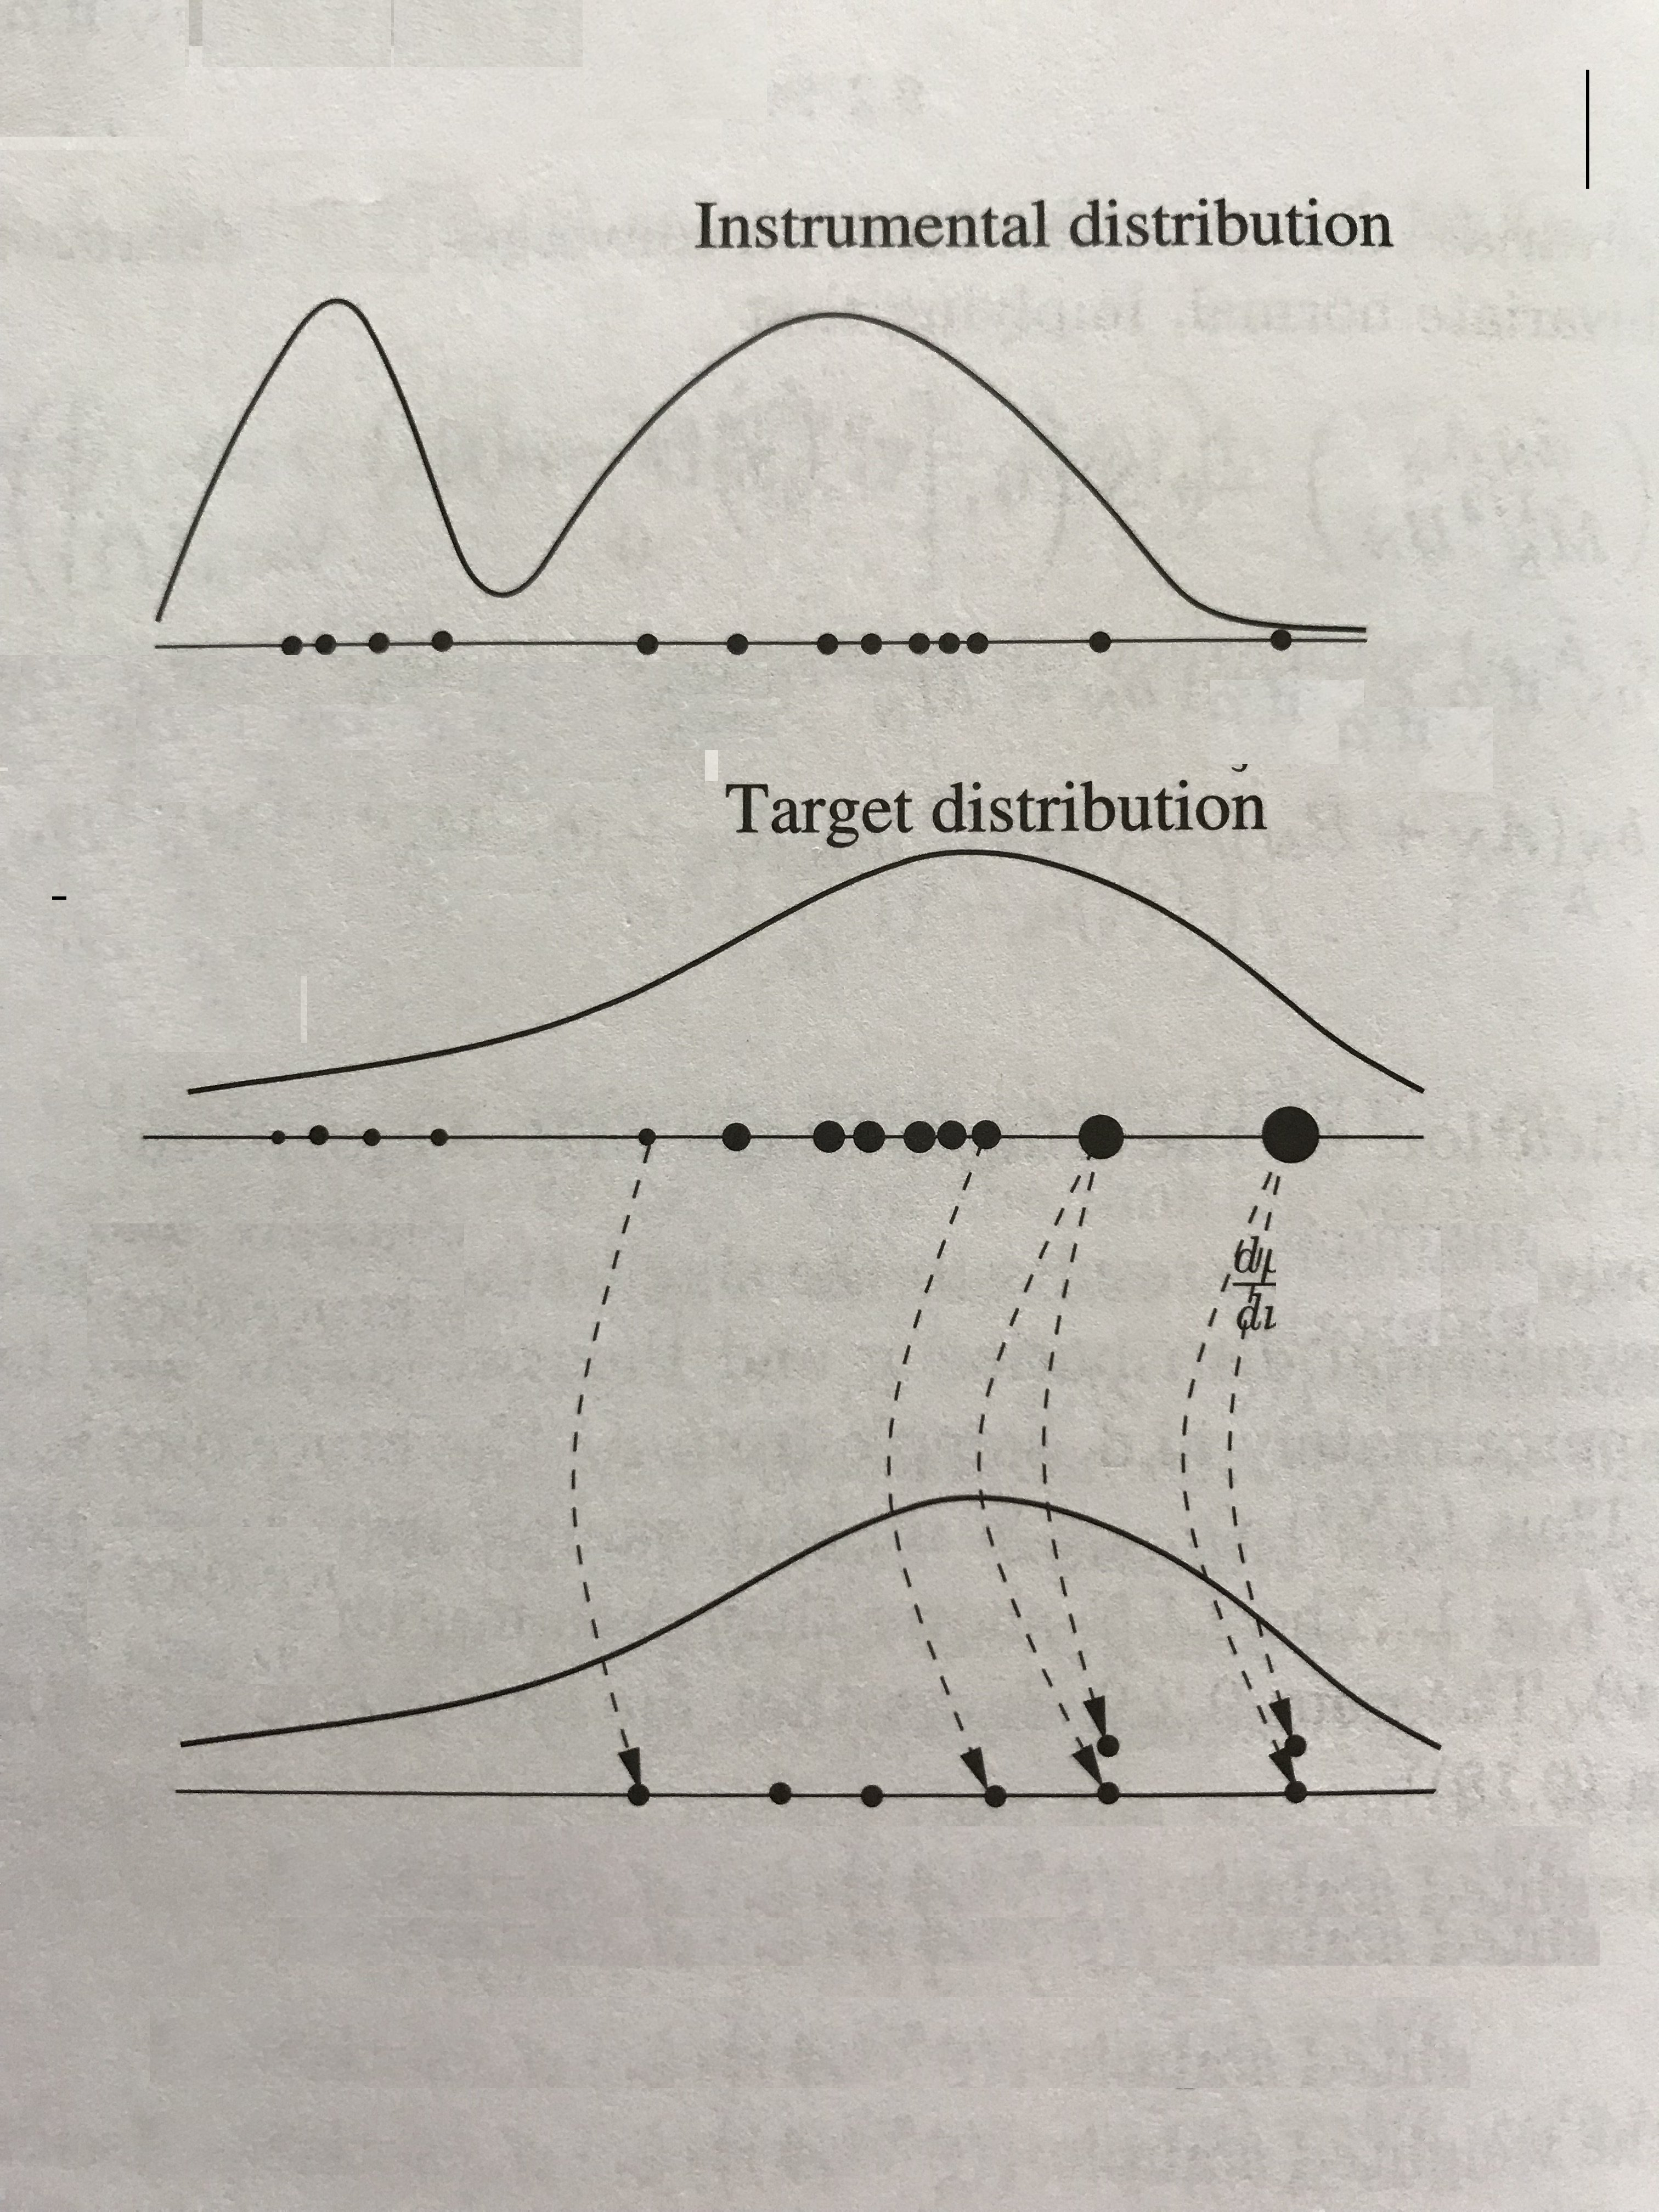
\includegraphics[width=50mm]{isr.jpg}
\end{center}
Original, unedited image is from \url{https://www.springer.com/us/book/9780387402642}

\end{frame}




% homework question: https://stats.stackexchange.com/questions/359977/conditional-expectation-on-an-estimator-for-defensive-sampling

%----------------------------------------------------------------------------------------
\begin{frame}[fragile]
\frametitle{SIR}


Stage 1: do importance sampling to get $\{ \theta^i, w(\theta^i) \}_{i=1}^S$.
\newline

Stage 2: for $i = 1, \ldots, S$, select 
$$
P[ \tilde{\theta}^i = \theta^j \mid \theta^1, w(\theta^1), \ldots, \theta^S, w(\theta^S) ] = \frac{w(\theta^j)}{ \sum_k w(\theta^k) }.
$$

\end{frame}

%----------------------------------------------------------------------------------------
\begin{frame}[fragile]
\frametitle{SIR}

Another way to write it:
\newline

Stage 1: do importance sampling to get $\{ \theta^i, w(\theta^i) \}_{i=1}^S$.
\newline

Stage 2: for $i = 1, \ldots, S$, select indexes
$$
P[ I^i = j \mid \theta^1, w(\theta^1), \ldots, \theta^S, w(\theta^S) ] = \frac{w(\theta^j)}{ \sum_k w(\theta^k) }
$$
and then set 
$$
\tilde{\theta}^i = \theta^{I^i}.
$$

\end{frame}


%----------------------------------------------------------------------------------------
\begin{frame}[fragile]
\frametitle{Example 2 revisited}

\begin{verbatim}
y <- 2 # fake data
log_unnorm_weight <- function(theta){ 
  # sqrt(2pi) because it will cancel out 
  -.5*(y - theta)^2 }
num_samples <- 10000
theta_draws <- rt(num_samples , 1)
lunws <- log_unnorm_weight(theta_draws)
# note: prob arg automatically normalizes
random_indexes <- sample(x = num_samples, 
                         size = num_samples, 
                         replace = T, 
                         prob = exp(lunws)) 
sort(random_indexes) # repeats!
resampled_draws <- theta_draws[random_indexes]
hist(resampled_draws) # can't do this unless we resample
\end{verbatim}

\end{frame}


%----------------------------------------------------------------------------------------
\section{Sequential Monte Carlo}
\begin{frame}[fragile]
\frametitle{Going sequential}

Resampling adds variance, so why do it?
\newline

It throws away bad samples, and duplicates promising ones. When you're looking at a sequence of distribution targets, this can have a good effect on future samples.
\pause
\newline

{\bf sequential monte carlo} or {\bf particle filtering} methods are basically doing SIR over and over again.

\end{frame}

%----------------------------------------------------------------------------------------
\begin{frame}[fragile]
\frametitle{Examples of sequences of distributions}

{\bf Data annealing} \footcite{Chopin}
\[
p(\theta), p(\theta \mid y_1), p(\theta \mid y_{1:2}), \ldots, p(\theta \mid y_{1:n}),
\]

{\bf Temperature annealing} \footcite{Neal}
\[
p(y \mid \theta)^{a_0} p(\theta), p(y \mid \theta)^{a_1} p(\theta),  \ldots p(y \mid \theta)^{a_n} p(\theta)
\]
with $0 = a_0 < a_1 < \cdots < a_n = 1$. 
\newline


{\bf filtering and smoothing} in state space models
\[
p(x_1 \mid y_1, \theta), \ldots , p(x_{n} \mid y_{1:n}, \theta)
\]

\end{frame}

%----------------------------------------------------------------------------------------
\begin{frame}[fragile]
\frametitle{state space models}

\tikzstyle{format} = [draw, thin, fill=blue!20]
\tikzstyle{medium} = [ellipse, draw, thin, fill=green!20, minimum height=2.5em]

\begin{figure}
\begin{tikzpicture}[node distance=3cm, auto,>=latex', thick]
    % We need to set at bounding box first. Otherwise the diagram
    % will change position for each frame.
    \path[use as bounding box] (-1,0) rectangle (10,-2);
    \path[->] node (past) { $\cdots$ };
    \path[->] node[format, right of=past] (xtm1) {$x_{t-1}$}
                  (past) edge node {$f_{t-1}$} (xtm1);
    \path[->] node[format, right of=xtm1] (xt) {$x_t$}
                  node[medium, below of=xtm1] (ytm1) { $Y_{t-1}$ }
                  (xtm1) edge node { $f_{t}$ } (xt)
                        edge node[swap] { $g_{t-1}$ } (ytm1);
    \path[->] node[right of=xt] (future) {$\cdots$}
                  node[medium, below of=xt] (yt) {$y_t$}
                  (xt) edge node {$f_{t+1}$} (future)
                       edge node[swap] {$g_{t}$} (yt);
\end{tikzpicture}
\end{figure}
% \vspace*{\baselineskip}
% \vspace*{\baselineskip}


\begin{align*}
&p(x_{1:T}, y_{1:T} \mid \theta) \\
&= g(y_1 \mid x_1, \theta) f(x_1 \mid \theta) \prod_{t=2}^T g(y_t \mid x_t, \theta) f(x_t \mid x_{t-1}, \theta)
\end{align*}

\end{frame}
%----------------------------------------------------------------------------------------
\begin{frame}[fragile]
\frametitle{Example: filtering in state space models}

Here's an example of a state space model. $y_t$ is a univariate time series, and $x_t$ is a hidden/unobserved/latent time series.
\newline

\begin{gather}
y_t = \exp(x_t / 2) \epsilon_t \\
x_t = c + \phi x_{t-1} + v_t
\end{gather}

We sometimes refer to (1) as $g(y_t \mid x_t, \theta)$ or the observation equation, and (2) as the state transition equation or $f(x_t \mid x_{t-1}, \theta)$.
\end{frame}

%----------------------------------------------------------------------------------------
\begin{frame}[fragile]
\frametitle{Example: filtering in state space models}

$y_{1:t}$ observed, $x_{1:t}$ hidden. Goal: $p(x_t \mid y_{1:t})$ in real-time.
\newline

\begin{center}
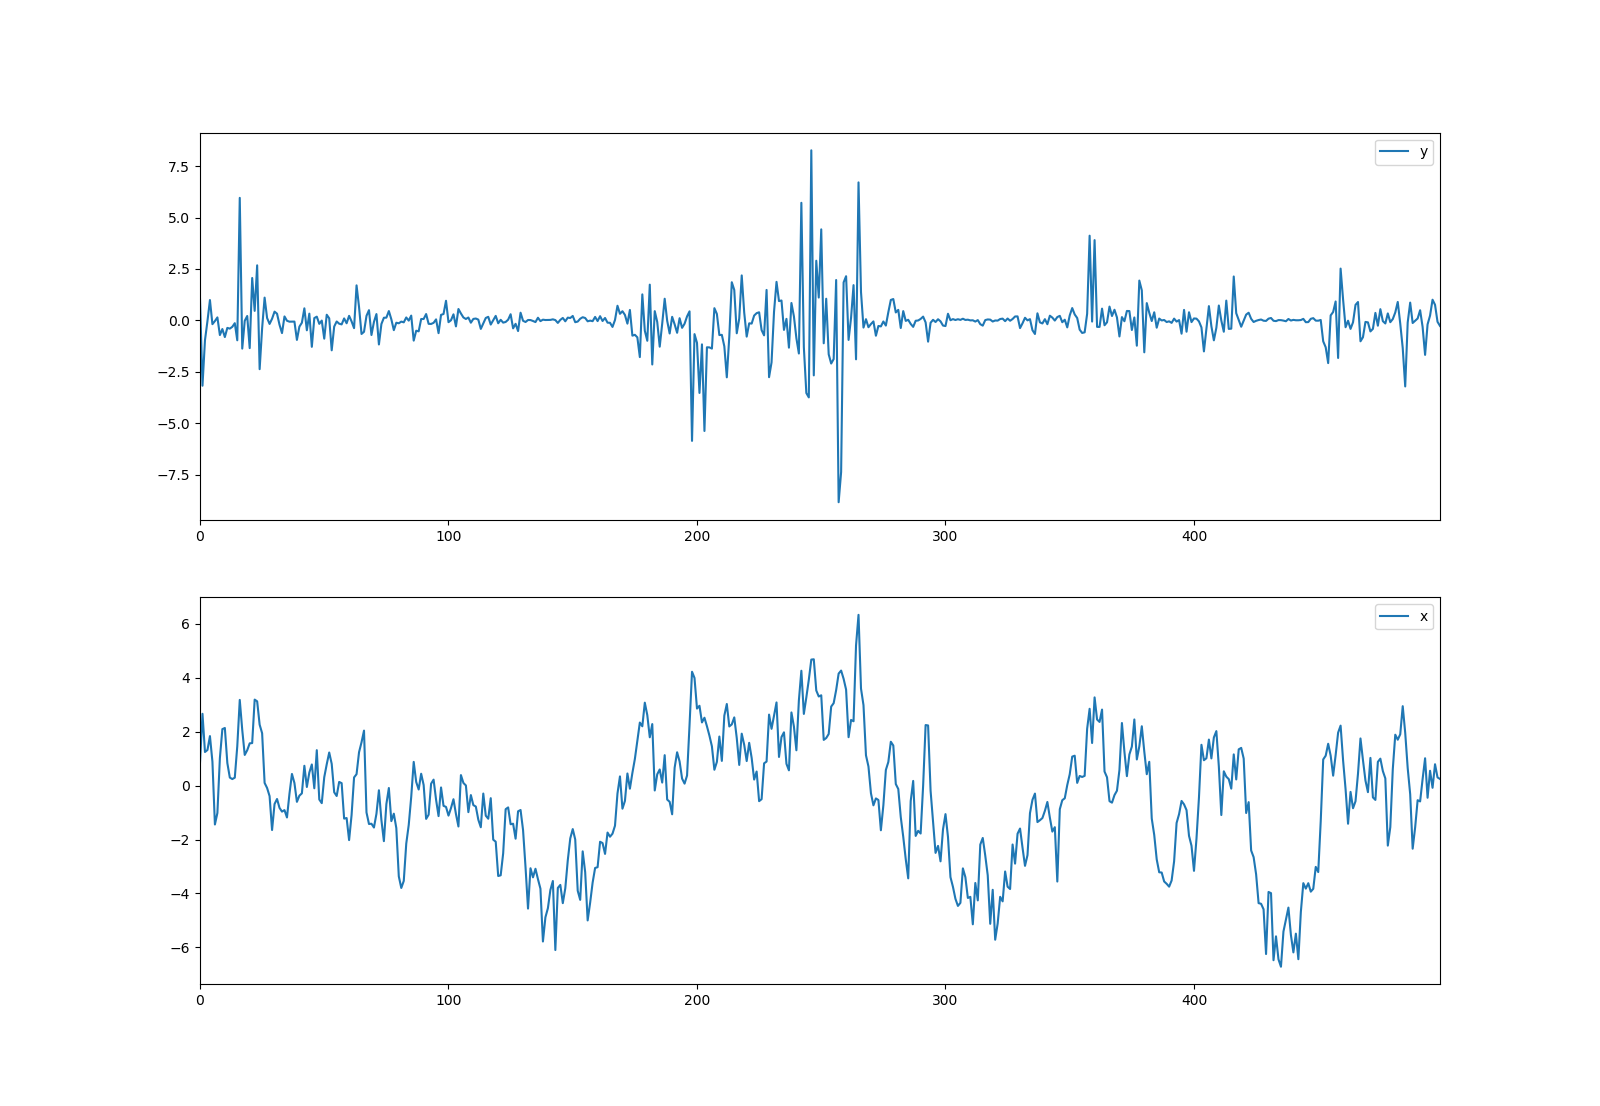
\includegraphics[width=103mm]{univ_svol_sim.png}
\end{center}

\end{frame}

%----------------------------------------------------------------------------------------
\begin{frame}[fragile]
\frametitle{Example: filtering in state space models}

\begin{center}
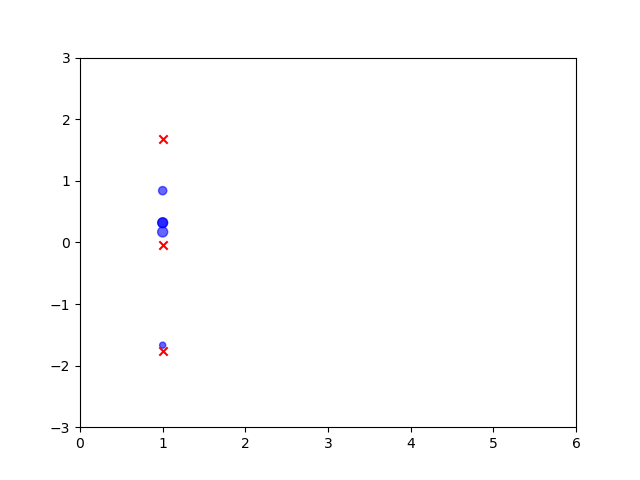
\includegraphics[width=80mm]{pfilt_anim_1.png}
\end{center}

\end{frame}

%----------------------------------------------------------------------------------------
\begin{frame}[fragile]
\frametitle{Going sequential}

\begin{center}
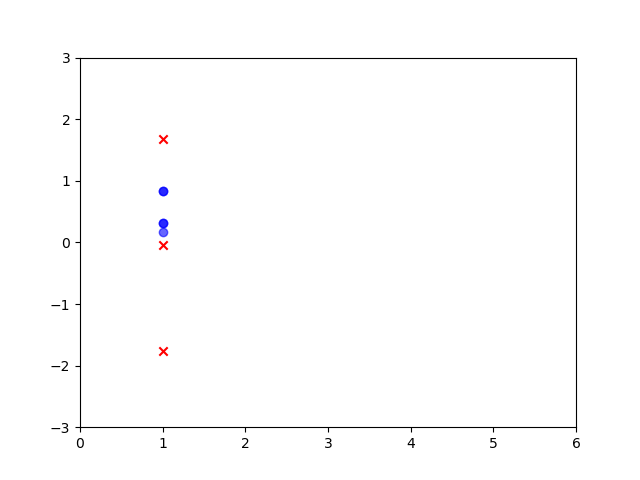
\includegraphics[width=80mm]{pfilt_anim_2.png}
\end{center}

\end{frame}

%----------------------------------------------------------------------------------------
\begin{frame}[fragile]
\frametitle{Going sequential}

\begin{center}
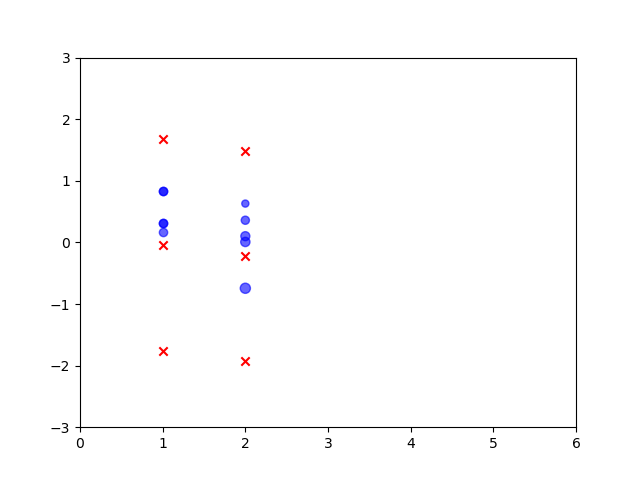
\includegraphics[width=80mm]{pfilt_anim_3.png}
\end{center}

\end{frame}
%----------------------------------------------------------------------------------------
\begin{frame}[fragile]
\frametitle{Going sequential}

\begin{center}
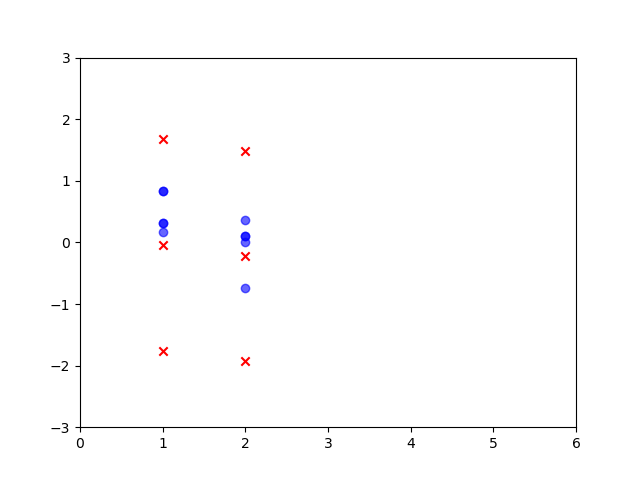
\includegraphics[width=80mm]{pfilt_anim_4.png}
\end{center}

\end{frame}
%----------------------------------------------------------------------------------------
\begin{frame}[fragile]
\frametitle{Going sequential}

\begin{center}
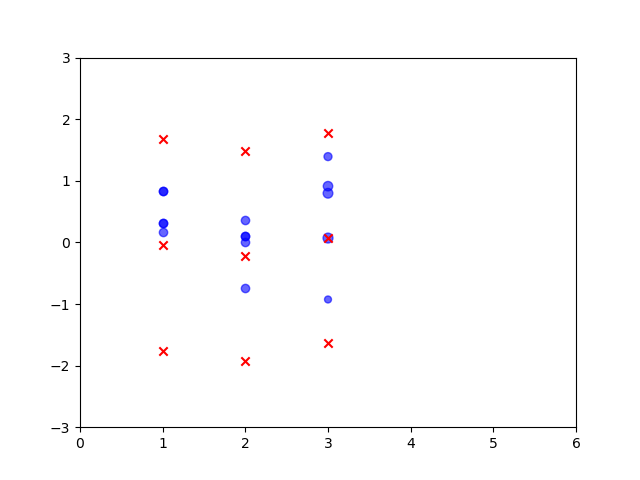
\includegraphics[width=80mm]{pfilt_anim_5.png}
\end{center}

\end{frame}
%----------------------------------------------------------------------------------------
\begin{frame}[fragile]
\frametitle{Going sequential}

\begin{center}
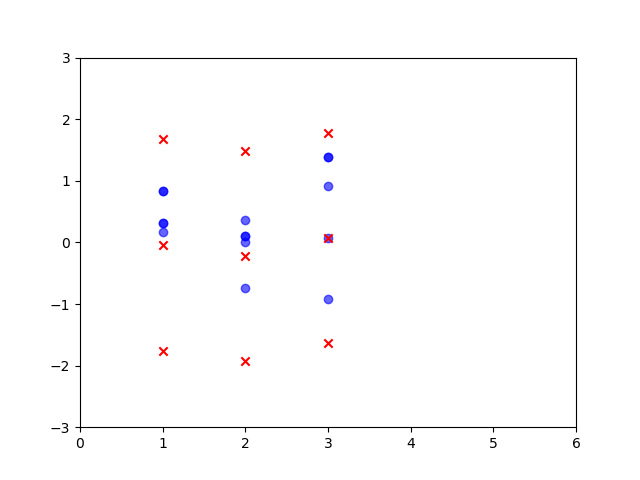
\includegraphics[width=80mm]{pfilt_anim_6.png}
\end{center}

\end{frame}
%----------------------------------------------------------------------------------------
\begin{frame}[fragile]
\frametitle{Going sequential}

\begin{center}
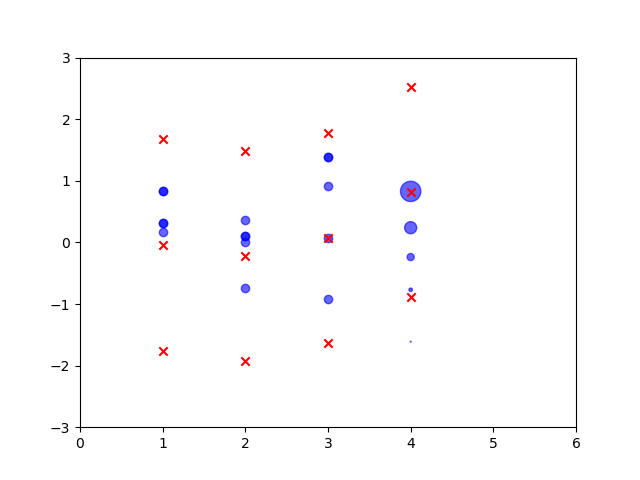
\includegraphics[width=80mm]{pfilt_anim_7.png}
\end{center}

\end{frame}
%----------------------------------------------------------------------------------------
\begin{frame}[fragile]
\frametitle{Going sequential}

\begin{center}
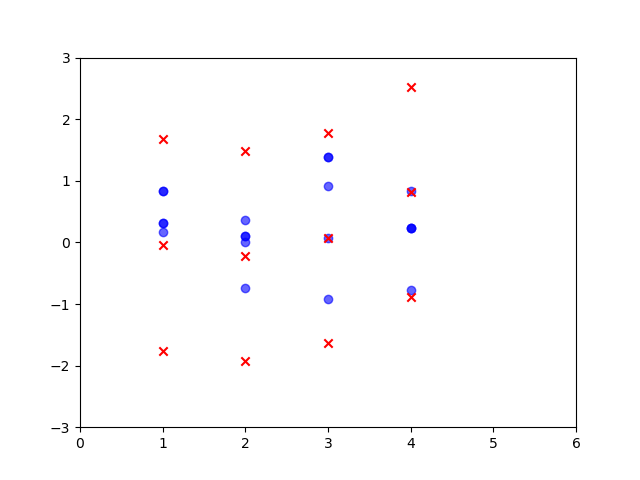
\includegraphics[width=80mm]{pfilt_anim_8.png}
\end{center}

\end{frame}
%----------------------------------------------------------------------------------------
\begin{frame}[fragile]
\frametitle{Going sequential}

\begin{center}
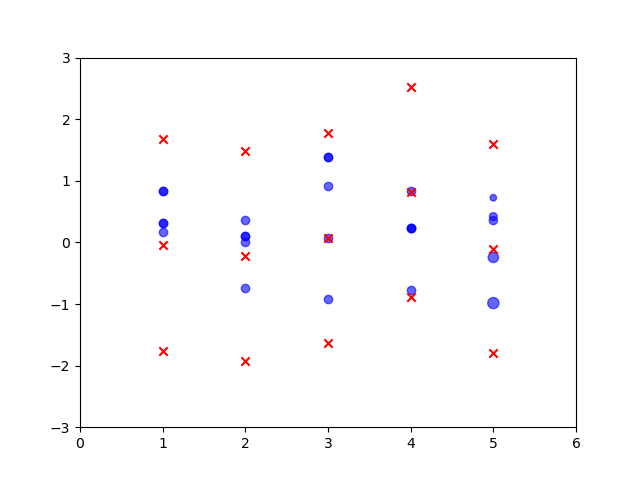
\includegraphics[width=80mm]{pfilt_anim_9.png}
\end{center}

\end{frame}
%----------------------------------------------------------------------------------------
\begin{frame}[fragile]
\frametitle{Going sequential}

\begin{center}
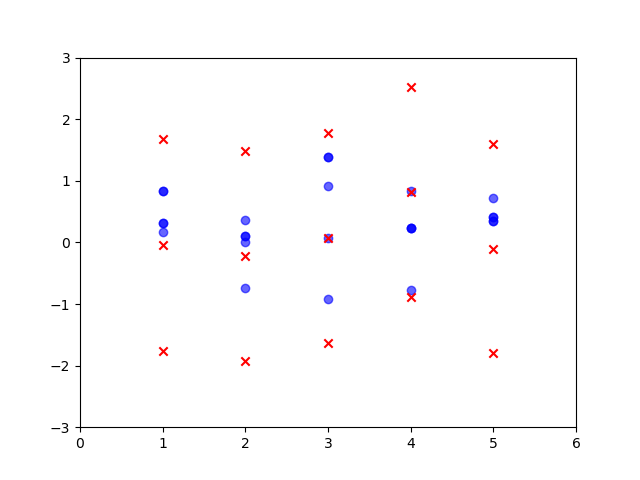
\includegraphics[width=80mm]{pfilt_anim_10.png}
\end{center}

\end{frame}




%----------------------------------------------------------------------------------------
\begin{frame}[fragile]
\frametitle{Filtering recursions}

Drop dependence on $\theta$ from the notation...
\begin{align*}
p(x_{1:t}|y_{1:t}) &=C_{t}^{-1} p(x_{t} , y_t  \mid x_{t-1})p(x_{1:t-1} \mid y_{1:t-1}) \\
&= C_{t}^{-1} \frac{p(x_t, y_t \mid x_{t-1})}{q_{t}(x_{t} \mid y_{t},x_{t-1})} \times \\
& \hspace{20mm} q_{t}(x_{t} \mid y_{t},x_{t-1})p(x_{1:t-1} \mid y_{1:t-1}) \\
&= C_{t}^{-1} \begingroup\color{red} \frac{g(y_t|x_t)f(x_t|x_{t-1})}{q_t(x_t|x_{t-1},y_t) } \endgroup \times \\
& \hspace{19mm} \begingroup\color{blue} q_t(x_t \mid x_{t-1},y_t) p(x_{1:t-1} \mid y_{1:t-1}) \endgroup\\
\end{align*}

Repeat through time:
\begin{enumerate}
\item start with samples from $p(x_{1:t-1} \mid y_{1:t-1})$
\item mutate/propogate/extend using $q_t(x_t \mid x_{t-1},y_t)$
\item adjust weights by multiplying by $ \begingroup\color{red} \frac{g(y_t|x_t)f(x_t|x_{t-1})}{q_t(x_t|x_{t-1},y_t) } \endgroup $
\item resample, giving you particles distributed as $p(x_{1:t} \mid y_{1:t})$
\end{enumerate}


\end{frame}


%----------------------------------------------------------------------------------------

\begin{frame}
\printbibliography
\end{frame}

\end{document} 



